% =====================================================================
%  Ovidius NIDS — Bachelor's Thesis Presentation
%  Beamer version (16:9 widescreen, Deep Navy + Cyan theme)
%
%  Author: Bora Cristian-Vasile
%  Advisor: Prof. Dorin Iordache
%  Universitatea Ovidius din Constanța, FMI, Computer Science
%  July 2026
%
%  Build:  pdflatex main.tex && pdflatex main.tex
%       or latexmk -pdf main.tex
% =====================================================================
\documentclass[aspectratio=169,11pt]{beamer}

% ----------- packages -----------
\usepackage[utf8]{inputenc}
\usepackage[T1]{fontenc}
\usepackage[english]{babel}
\usepackage{lmodern}
\usepackage{microtype}
\usepackage{tikz}
\usepackage{xcolor}
\usepackage{pifont}      % \ding{52} = check, \ding{55} = cross
\usepackage{booktabs}
\usepackage{colortbl}    % \rowcolor
\usepackage{array}
\usepackage{tabularx}
\usepackage{calc}
\usetikzlibrary{shapes.geometric,arrows.meta,positioning,backgrounds,fit}

% ----------- color palette (matches the SIEM console + PPTX) -----------
\definecolor{navybg}{HTML}{0A1220}     % slide background
\definecolor{navysurface}{HTML}{111B30}% card background
\definecolor{navy2}{HTML}{162241}      % raised card
\definecolor{navyborder}{HTML}{1A2D4F} % hairlines
\definecolor{textmain}{HTML}{E2E8F0}   % primary text
\definecolor{textmute}{HTML}{94A3B8}   % muted text
\definecolor{textdim}{HTML}{64748B}    % captions
\definecolor{cyan2}{HTML}{22D3EE}      % primary accent
\definecolor{fuchsia2}{HTML}{D946EF}   % ML accent
\definecolor{amber2}{HTML}{F59E0B}     % attacks
\definecolor{green2}{HTML}{10B981}     % success
\definecolor{red2}{HTML}{EF4444}       % critical
\definecolor{blue2}{HTML}{38BDF8}      % info

% ----------- beamer theme setup -----------
\setbeamercolor{background canvas}{bg=navybg}
\setbeamercolor{normal text}{fg=textmain,bg=navybg}
\setbeamercolor{frametitle}{fg=textmain,bg=navybg}
\setbeamercolor{title}{fg=textmain}
\setbeamercolor{subtitle}{fg=cyan2}
\setbeamercolor{structure}{fg=cyan2}
\setbeamercolor{itemize item}{fg=cyan2}
\setbeamercolor{itemize subitem}{fg=cyan2}
\setbeamercolor{block title}{fg=textmain,bg=navy2}
\setbeamercolor{block body}{fg=textmain,bg=navysurface}
\setbeamercolor{author}{fg=textmute}
\setbeamercolor{institute}{fg=textmute}
\setbeamercolor{date}{fg=textdim}

\setbeamerfont{frametitle}{series=\bfseries,size=\Large}
\setbeamerfont{title}{series=\bfseries,size=\huge}
\setbeamerfont{subtitle}{shape=\itshape,size=\large}
\setbeamerfont{normal text}{size=\normalsize}

% Remove navigation symbols
\setbeamertemplate{navigation symbols}{}

% Custom frame title with kicker line
\setbeamertemplate{frametitle}{%
  \vspace{0.6em}\hspace{0.6em}%
  \begin{minipage}{\dimexpr\paperwidth-1.2em\relax}
    {\color{cyan2}\bfseries\fontsize{8.5}{10}\selectfont\MakeUppercase{\insertframesubtitle}}\\[0.15em]
    {\color{textmain}\bfseries\Large\insertframetitle}
  \end{minipage}%
  \vspace{0.3em}
}

% Custom footer
\setbeamertemplate{footline}{%
  \leavevmode%
  \hbox{%
    \begin{beamercolorbox}[wd=\paperwidth,ht=2.2ex,dp=1ex,leftskip=0.6em,rightskip=0.6em]{normal text}%
      \color{textdim}\fontsize{7}{8}\selectfont Ovidius NIDS · Bora Cristian-Vasile · \insertframenumber/\inserttotalframenumber
    \end{beamercolorbox}%
  }%
}

% ------ macros for repeated patterns ------
\newcommand{\kicker}[1]{{\color{cyan2}\bfseries\fontsize{8.5}{10}\selectfont\MakeUppercase{#1}}}
\newcommand{\tmono}[1]{{\ttfamily\small\color{textmain} #1}}
\newcommand{\tagchip}[2]{%
  \tikz[baseline=(c.base)]\node[fill=#1!12,draw=#1,line width=0.4pt,
    rounded corners=2pt,inner xsep=4pt,inner ysep=1.5pt,
    text=#1,font=\bfseries\fontsize{7}{8}\selectfont]
  (c) {\strut\MakeUppercase{#2}};
}

% A reusable "tile" environment that simulates the PPTX cards.
% Usage:  \tile{accentcolor}{title}{body}
\newcommand{\tile}[3]{%
  \begin{tikzpicture}
    \node[draw=navyborder,fill=navysurface,line width=0.5pt,
          rounded corners=1pt,inner sep=8pt,
          minimum width=0.96\linewidth,minimum height=2.6cm,
          text width=0.88\linewidth,align=left] (t) {
      {\color{#1}\bfseries\large #2}\\[2pt]
      {\color{textmute}\small #3}
    };
    \draw[line width=2pt,#1] (t.north west) -- (t.south west);
  \end{tikzpicture}%
}
% Compact tile variant for 3- and 4-column layouts (smaller text + height)
\newcommand{\smalltile}[3]{%
  \begin{tikzpicture}
    \node[draw=navyborder,fill=navysurface,line width=0.5pt,
          rounded corners=1pt,inner sep=6pt,
          minimum width=0.96\linewidth,minimum height=2.2cm,
          text width=0.88\linewidth,align=left] (t) {
      {\color{#1}\bfseries\normalsize #2}\\[2pt]
      {\color{textmute}\fontsize{8}{10}\selectfont #3}
    };
    \draw[line width=1.5pt,#1] (t.north west) -- (t.south west);
  \end{tikzpicture}%
}

% ----------- document metadata -----------
\title{Information System for Network Detection Intrusion}
\subtitle{}
\author{Bora Cristian-Vasile}
\institute{Universitatea OVIDIUS din Constanța\\Facultatea de Matematică și Informatică\\Computer Science}
\date{Iulie 2026}

% =====================================================================
\begin{document}

% --------------------------------------------------------------------
% SLIDE 1 — Title
% --------------------------------------------------------------------
{
\setbeamertemplate{footline}{}
\begin{frame}[plain]
  \vspace{0.4em}
  \begin{columns}[T]
    \column{0.22\textwidth}
    \begin{tikzpicture}
      \node[anchor=north west,inner sep=0] at (0,0)
        {
\includegraphics[width=2.4cm]{ovidius-logo.png}};
    \end{tikzpicture}
    \column{0.74\textwidth}
    {\color{textmute}\small\bfseries\setlength{\baselineskip}{1.4em}
     OVIDIUS UNIVERSITY OF CONSTANȚA\\
     {\color{textdim}\mdseries Faculty of Mathematics and Computer Science  \,$\cdot$\,
      Computer Science}}
  \end{columns}
  \vspace{1.6em}

  \begin{center}
    \tikz \draw[cyan2,line width=1.5pt] (0,0) -- (12.8,0);
  \end{center}
  \vspace{0.5em}

  \begin{center}
    {\color{cyan2}\bfseries\large\MakeUppercase{Bachelor's Thesis}}\\[0.6em]
    {\color{textmain}\bfseries\fontsize{28}{34}\selectfont
     Information System for\\
     Network Detection Intrusion}
  \end{center}
  \vfill

  \begin{columns}[T]
    \column{0.5\textwidth}
    \kicker{Graduate}\\[0.2em]
    {\color{textmain}\bfseries\large Bora Cristian-Vasile}
    \column{0.5\textwidth}
    \hfill\begin{minipage}{0.95\linewidth}
    \kicker{Scientific Advisor}\\[0.2em]
    {\color{textmain}\bfseries\large Prof. Dorin Iordache}
    \end{minipage}
  \end{columns}
  \vspace{0.8em}

  \begin{center}
    {\color{textdim}\small Constanța \,$\cdot$\, July 2026}
  \end{center}
\end{frame}
}

% --------------------------------------------------------------------
% SLIDE 2 — Purpose
% --------------------------------------------------------------------
\begin{frame}
  \frametitle{Project purpose}
  \framesubtitle{01 · Purpose}

  \vspace{0.4em}
  \begin{columns}[T,onlytextwidth]
    \column{0.49\textwidth}
    \tile{cyan2}{\ding{125}~Real-time detection}{%
      Each packet inspected as it arrives. No PCAP files analysed offline.}
    \vspace{0.6em}
    \tile{amber2}{\ding{73}~Built-in forensics}{%
      Per alert: a snapshot of the last 50 packets, downloadable from the UI.}

    \column{0.49\textwidth}
    \tile{fuchsia2}{\ding{72}~Hybrid signatures + ML}{%
      Two complementary engines. When both agree, the alert gets the hybrid label.}
    \vspace{0.6em}
    \tile{green2}{\ding{229}~Easy demo}{%
      One-click launcher: auto-install, FastAPI + Vite start, browser opens.}
  \end{columns}
\end{frame}

% --------------------------------------------------------------------
% SLIDE 3 — Idea
% --------------------------------------------------------------------
\begin{frame}
  \frametitle{Project idea}
  \framesubtitle{02 · Idea}

  \vspace{0.2em}
  {\color{textmute}\itshape Neither classical paradigm solves the problem on its own.}
  \vspace{0.6em}

  \begin{columns}[T,onlytextwidth]
    \column{0.32\textwidth}
    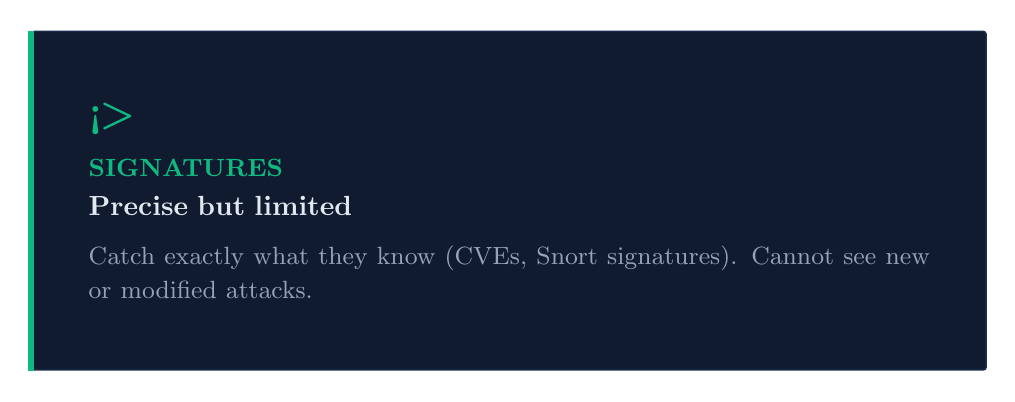
\begin{tikzpicture}
      \node[draw=navyborder,fill=navysurface,line width=0.5pt,
            rounded corners=1pt,inner sep=10pt,
            minimum width=\linewidth,minimum height=4.3cm,
            text width=0.88\linewidth,align=left] (t) {
        {\color{green2}\Large\textbf{<\hspace{-1pt}\textgreater}}\\[6pt]
        {\color{green2}\bfseries\small\MakeUppercase{Signatures}}\\[2pt]
        {\color{textmain}\bfseries\normalsize Precise but limited}\\[6pt]
        {\color{textmute}\small Catch exactly what they know (CVEs, Snort signatures). Cannot see new or modified attacks.}
      };
      \draw[line width=2.2pt,green2] (t.north west) -- (t.south west);
    \end{tikzpicture}

    \column{0.32\textwidth}
    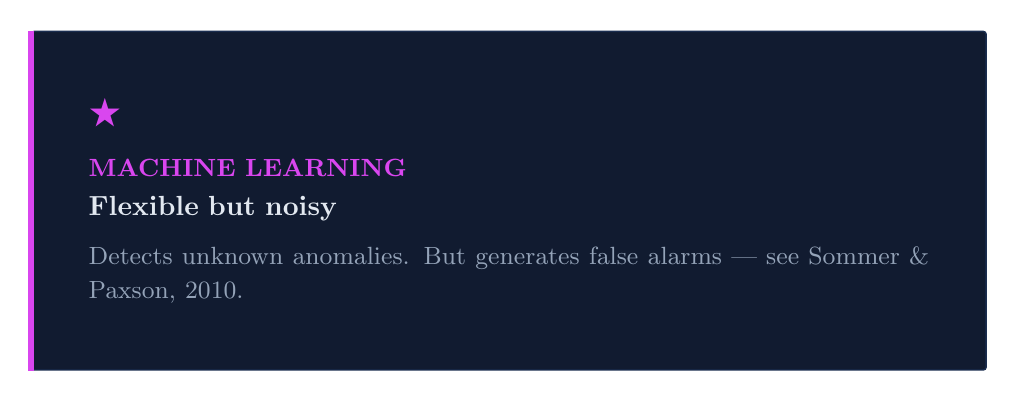
\begin{tikzpicture}
      \node[draw=navyborder,fill=navysurface,line width=0.5pt,
            rounded corners=1pt,inner sep=10pt,
            minimum width=\linewidth,minimum height=4.3cm,
            text width=0.88\linewidth,align=left] (t) {
        {\color{fuchsia2}\Large\ding{72}}\\[6pt]
        {\color{fuchsia2}\bfseries\small\MakeUppercase{Machine Learning}}\\[2pt]
        {\color{textmain}\bfseries\normalsize Flexible but noisy}\\[6pt]
        {\color{textmute}\small Detects unknown anomalies. But generates false alarms — see Sommer \& Paxson, 2010.}
      };
      \draw[line width=2.2pt,fuchsia2] (t.north west) -- (t.south west);
    \end{tikzpicture}

    \column{0.32\textwidth}
    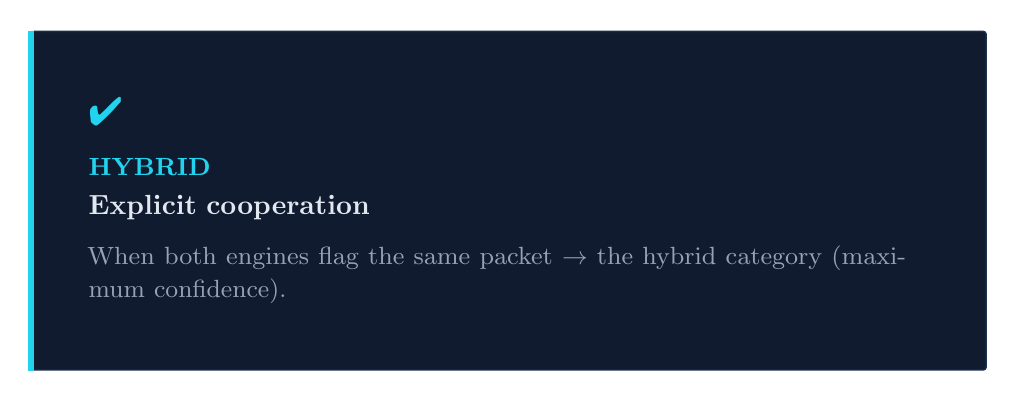
\begin{tikzpicture}
      \node[draw=navyborder,fill=navysurface,line width=0.5pt,
            rounded corners=1pt,inner sep=10pt,
            minimum width=\linewidth,minimum height=4.3cm,
            text width=0.88\linewidth,align=left] (t) {
        {\color{cyan2}\Large\ding{52}}\\[6pt]
        {\color{cyan2}\bfseries\small\MakeUppercase{Hybrid}}\\[2pt]
        {\color{textmain}\bfseries\normalsize Explicit cooperation}\\[6pt]
        {\color{textmute}\small When both engines flag the same packet $\rightarrow$ the hybrid category (maximum confidence).}
      };
      \draw[line width=2.2pt,cyan2] (t.north west) -- (t.south west);
    \end{tikzpicture}
  \end{columns}

  \vspace{0.6em}
  \begin{center}
  
\begin{tikzpicture}
    \node[draw=cyan2,fill=navysurface,line width=0.7pt,rounded corners=1pt,
          inner sep=7pt,text width=0.92\textwidth,align=center,
          font=\itshape] {
      {\color{textmain}Plus a built-in forensics layer — every alert keeps the context of the packets that triggered it.}
    };
  \end{tikzpicture}
  \end{center}
\end{frame}

% --------------------------------------------------------------------
% SLIDE 4 — Technologies
% --------------------------------------------------------------------
\begin{frame}
  \frametitle{Technologies used}
  \framesubtitle{03 · Technologies}

  \begin{columns}[T,onlytextwidth]
    \column{0.49\textwidth}
    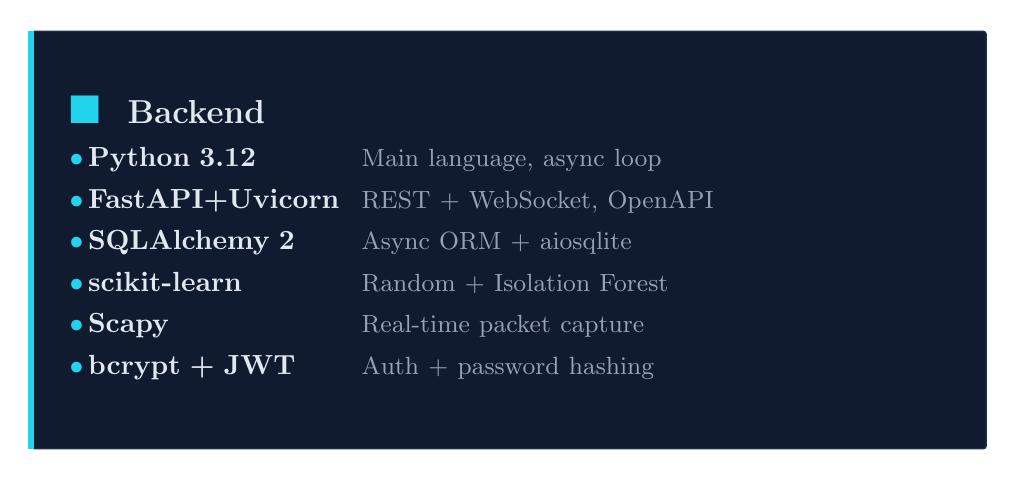
\begin{tikzpicture}
      \node[draw=navyborder,fill=navysurface,line width=0.5pt,rounded corners=1pt,
            inner sep=10pt,minimum width=\linewidth,minimum height=5.3cm,
            text width=0.92\linewidth,align=left] (t) {
        {\color{cyan2}\Large\ding{110}}\quad{\color{textmain}\bfseries\large Backend}\\[6pt]
        \begin{tabular}{@{}l@{\hspace{0.8em}}l@{}}
          {\color{cyan2}$\bullet$}\,{\color{textmain}\bfseries Python 3.12}      & {\color{textmute}\small Main language, async loop} \\[3pt]
          {\color{cyan2}$\bullet$}\,{\color{textmain}\bfseries FastAPI+Uvicorn}  & {\color{textmute}\small REST + WebSocket, OpenAPI}\\[3pt]
          {\color{cyan2}$\bullet$}\,{\color{textmain}\bfseries SQLAlchemy 2}     & {\color{textmute}\small Async ORM + aiosqlite}    \\[3pt]
          {\color{cyan2}$\bullet$}\,{\color{textmain}\bfseries scikit-learn}     & {\color{textmute}\small Random + Isolation Forest} \\[3pt]
          {\color{cyan2}$\bullet$}\,{\color{textmain}\bfseries Scapy}            & {\color{textmute}\small Real-time packet capture} \\[3pt]
          {\color{cyan2}$\bullet$}\,{\color{textmain}\bfseries bcrypt + JWT}     & {\color{textmute}\small Auth + password hashing} \\
        \end{tabular}
      };
      \draw[line width=2.2pt,cyan2] (t.north west) -- (t.south west);
    \end{tikzpicture}

    \column{0.49\textwidth}
    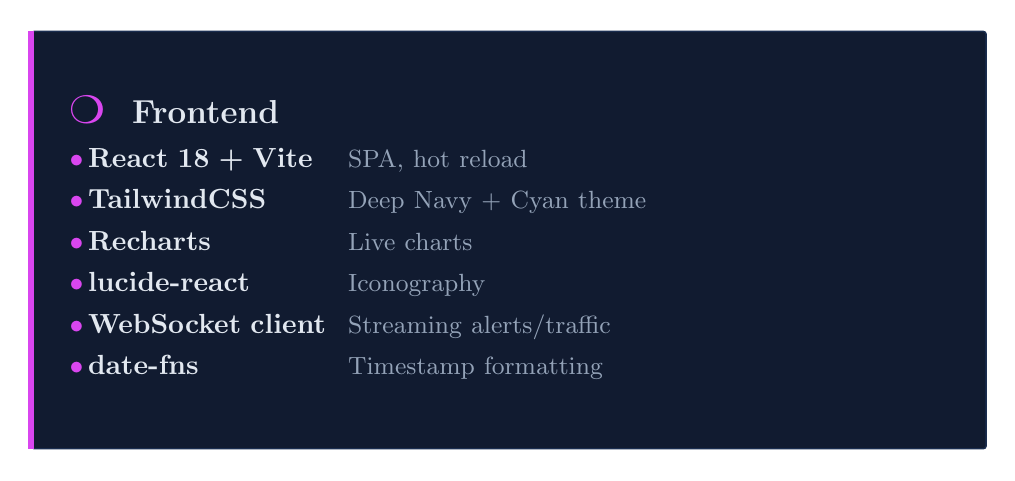
\begin{tikzpicture}
      \node[draw=navyborder,fill=navysurface,line width=0.5pt,rounded corners=1pt,
            inner sep=10pt,minimum width=\linewidth,minimum height=5.3cm,
            text width=0.92\linewidth,align=left] (t) {
        {\color{fuchsia2}\Large\ding{109}}\quad{\color{textmain}\bfseries\large Frontend}\\[6pt]
        \begin{tabular}{@{}l@{\hspace{0.8em}}l@{}}
          {\color{fuchsia2}$\bullet$}\,{\color{textmain}\bfseries React 18 + Vite}    & {\color{textmute}\small SPA, hot reload}        \\[3pt]
          {\color{fuchsia2}$\bullet$}\,{\color{textmain}\bfseries TailwindCSS}        & {\color{textmute}\small Deep Navy + Cyan theme} \\[3pt]
          {\color{fuchsia2}$\bullet$}\,{\color{textmain}\bfseries Recharts}           & {\color{textmute}\small Live charts}           \\[3pt]
          {\color{fuchsia2}$\bullet$}\,{\color{textmain}\bfseries lucide-react}       & {\color{textmute}\small Iconography}           \\[3pt]
          {\color{fuchsia2}$\bullet$}\,{\color{textmain}\bfseries WebSocket client}   & {\color{textmute}\small Streaming alerts/traffic}\\[3pt]
          {\color{fuchsia2}$\bullet$}\,{\color{textmain}\bfseries date-fns}           & {\color{textmute}\small Timestamp formatting} \\
        \end{tabular}
      };
      \draw[line width=2.2pt,fuchsia2] (t.north west) -- (t.south west);
    \end{tikzpicture}
  \end{columns}
\end{frame}

% --------------------------------------------------------------------
% SLIDE 5 — Architecture
% --------------------------------------------------------------------
\begin{frame}
  \frametitle{Packet flow through the system}
  \framesubtitle{04 · Architecture}

  \vspace{0.2em}
  \begin{center}
    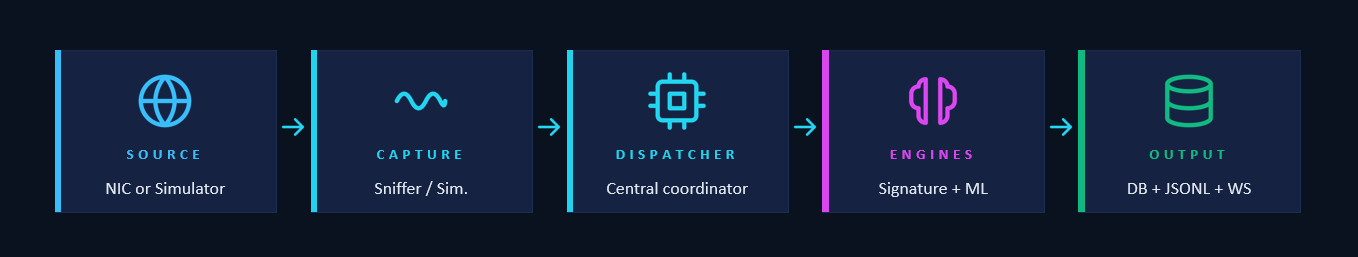
\includegraphics[width=0.97\textwidth]{architecture-diagram.png}
  \end{center}

  \vspace{0.4em}
  \begin{columns}[T,onlytextwidth]
    \column{0.245\textwidth}
    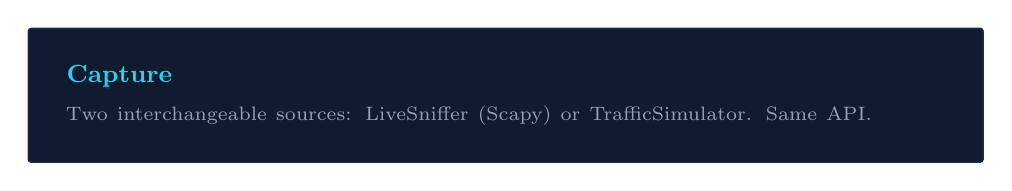
\begin{tikzpicture}
      \node[draw=navyborder,fill=navysurface,line width=0.5pt,rounded corners=1pt,
            inner sep=6pt,minimum width=\linewidth,minimum height=1.7cm,
            text width=0.92\linewidth,align=left] {
        {\color{cyan2}\bfseries\small Capture}\\[2pt]
        {\color{textmute}\fontsize{7.5}{9}\selectfont Two interchangeable sources: LiveSniffer (Scapy) or TrafficSimulator. Same API.}
      };
    \end{tikzpicture}
    \column{0.245\textwidth}
    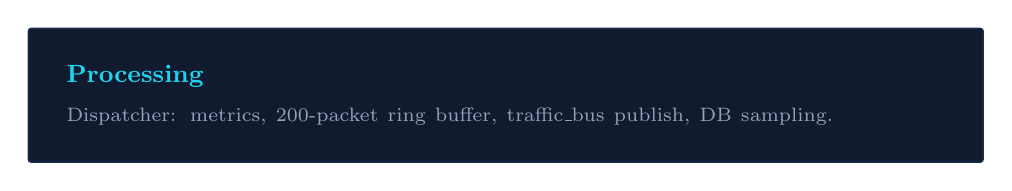
\begin{tikzpicture}
      \node[draw=navyborder,fill=navysurface,line width=0.5pt,rounded corners=1pt,
            inner sep=6pt,minimum width=\linewidth,minimum height=1.7cm,
            text width=0.92\linewidth,align=left] {
        {\color{cyan2}\bfseries\small Processing}\\[2pt]
        {\color{textmute}\fontsize{7.5}{9}\selectfont Dispatcher: metrics, 200-packet ring buffer, traffic\_bus publish, DB sampling.}
      };
    \end{tikzpicture}
    \column{0.245\textwidth}
    
\begin{tikzpicture}
      \node[draw=navyborder,fill=navysurface,line width=0.5pt,rounded corners=1pt,
            inner sep=6pt,minimum width=\linewidth,minimum height=1.7cm,
            text width=0.92\linewidth,align=left] {
        {\color{cyan2}\bfseries\small Detection}\\[2pt]
        {\color{textmute}\fontsize{7.5}{9}\selectfont Signature engine (10 YAML rules) + ML scoring. Three categories.}
      };
    \end{tikzpicture}
    \column{0.245\textwidth}
    
\begin{tikzpicture}
      \node[draw=navyborder,fill=navysurface,line width=0.5pt,rounded corners=1pt,
            inner sep=6pt,minimum width=\linewidth,minimum height=1.7cm,
            text width=0.92\linewidth,align=left] {
        {\color{cyan2}\bfseries\small Persistence}\\[2pt]
        {\color{textmute}\fontsize{7.5}{9}\selectfont Alerts in SQLite + JSONL per alert on disk. Broadcast on alert\_bus.}
      };
    \end{tikzpicture}
  \end{columns}

  \vspace{0.4em}
  \begin{center}\color{green2}\itshape\small
    End-to-end latency (packet $\rightarrow$ UI notification) under 250 ms on a laptop.
  \end{center}
\end{frame}

% --------------------------------------------------------------------
% SLIDE 6 — Components
% --------------------------------------------------------------------
\begin{frame}
  \frametitle{The modules that make up the application}
  \framesubtitle{05 · Components}

  \begin{columns}[T,onlytextwidth]
    \column{0.32\textwidth}
    \tile{cyan2}{\ding{125}~Sniffer / Simulator}{Real packet capture (Scapy) or synthetic generation for demos.}
    \vspace{0.4em}
    \tile{fuchsia2}{\ding{72}~ML Detector}{Random Forest or Isolation Forest on 6 features per packet.}

    \column{0.32\textwidth}
    \tile{cyan2}{\ding{110}~Dispatcher}{The central point. Coordinates metrics, engines, persistence, broadcast.}
    \vspace{0.4em}
    \tile{amber2}{\ding{73}~Forensics}{200-packet ring buffer; per alert, JSONL written to disk.}

    \column{0.32\textwidth}
    \tile{green2}{\ding{52}~Signature Engine}{Editable rules: protocol, IP, port, content, regex, threshold.}
    \vspace{0.4em}
    \tile{blue2}{\ding{109}~API + WebSocket}{JWT-protected REST + /ws/alerts + /ws/traffic streaming.}
  \end{columns}
\end{frame}

% --------------------------------------------------------------------
% SLIDE 7 — Implementation: pipeline
% --------------------------------------------------------------------
\begin{frame}
  \frametitle{The detection pipeline}
  \framesubtitle{06 · Implementation}

  \begin{columns}[T,onlytextwidth]
    \column{0.55\textwidth}
    {\color{cyan2}\bfseries\large Per-packet processing}\\[4pt]
    \begin{tabular}{@{}p{1.1em}@{\hspace{4pt}}p{0.86\linewidth}@{}}
      \tikz\node[circle,fill=cyan2,text=navybg,inner sep=1pt,minimum size=1.1em,font=\bfseries\fontsize{7}{8}\selectfont]{1}; & {\color{textmain}\small \tmono{Dispatcher.handle(pkt)} on every captured packet.}\\[3pt]
      \tikz\node[circle,fill=cyan2,text=navybg,inner sep=1pt,minimum size=1.1em,font=\bfseries\fontsize{7}{8}\selectfont]{2}; & {\color{textmain}\small Increment counters + update PPS (1\,s sliding window).}\\[3pt]
      \tikz\node[circle,fill=cyan2,text=navybg,inner sep=1pt,minimum size=1.1em,font=\bfseries\fontsize{7}{8}\selectfont]{3}; & {\color{textmain}\small Packet enters the 200-slot ring buffer.}\\[3pt]
      \tikz\node[circle,fill=cyan2,text=navybg,inner sep=1pt,minimum size=1.1em,font=\bfseries\fontsize{7}{8}\selectfont]{4}; & {\color{textmain}\small Publish on \tmono{traffic\_bus} $\rightarrow$ live dashboard chart.}\\[3pt]
      \tikz\node[circle,fill=cyan2,text=navybg,inner sep=1pt,minimum size=1.1em,font=\bfseries\fontsize{7}{8}\selectfont]{5}; & {\color{textmain}\small 1/5 sampling persisted as TrafficEvent.}\\[3pt]
      \tikz\node[circle,fill=cyan2,text=navybg,inner sep=1pt,minimum size=1.1em,font=\bfseries\fontsize{7}{8}\selectfont]{6}; & {\color{textmain}\small Signature engine iterates the compiled rules (10 default).}\\[3pt]
      \tikz\node[circle,fill=cyan2,text=navybg,inner sep=1pt,minimum size=1.1em,font=\bfseries\fontsize{7}{8}\selectfont]{7}; & {\color{textmain}\small ML detector extracts features and scores the packet.}\\[3pt]
      \tikz\node[circle,fill=cyan2,text=navybg,inner sep=1pt,minimum size=1.1em,font=\bfseries\fontsize{7}{8}\selectfont]{8}; & {\color{textmain}\small Merge: signature-only, ml-only or hybrid $\rightarrow$ alerts.}\\
    \end{tabular}

    \column{0.42\textwidth}
    {\color{cyan2}\bfseries\large Alert categories}\\[4pt]

    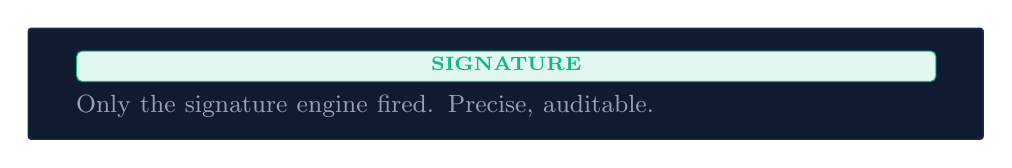
\begin{tikzpicture}
      \node[draw=navyborder,fill=navysurface,line width=0.5pt,rounded corners=1pt,
            inner sep=8pt,minimum width=\linewidth,
            text width=0.9\linewidth,align=left] {
        \tagchip{green2}{signature}\\[3pt]
        {\color{textmute}\small Only the signature engine fired. Precise, auditable.}
      };
    \end{tikzpicture}
    \vspace{0.4em}

    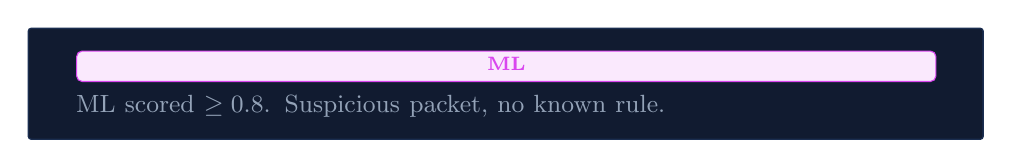
\begin{tikzpicture}
      \node[draw=navyborder,fill=navysurface,line width=0.5pt,rounded corners=1pt,
            inner sep=8pt,minimum width=\linewidth,
            text width=0.9\linewidth,align=left] {
        \tagchip{fuchsia2}{ml}\\[3pt]
        {\color{textmute}\small ML scored $\ge 0.8$. Suspicious packet, no known rule.}
      };
    \end{tikzpicture}
    \vspace{0.4em}

    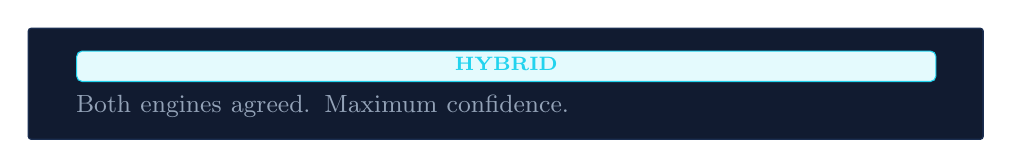
\begin{tikzpicture}
      \node[draw=navyborder,fill=navysurface,line width=0.5pt,rounded corners=1pt,
            inner sep=8pt,minimum width=\linewidth,
            text width=0.9\linewidth,align=left] {
        \tagchip{cyan2}{hybrid}\\[3pt]
        {\color{textmute}\small Both engines agreed. Maximum confidence.}
      };
    \end{tikzpicture}
  \end{columns}
\end{frame}

% --------------------------------------------------------------------
% SLIDE 8 — Machine Learning
% --------------------------------------------------------------------
\begin{frame}
  \frametitle{Two complementary algorithms}
  \framesubtitle{07 · Machine Learning}

  \begin{columns}[T,onlytextwidth]
    \column{0.49\textwidth}
    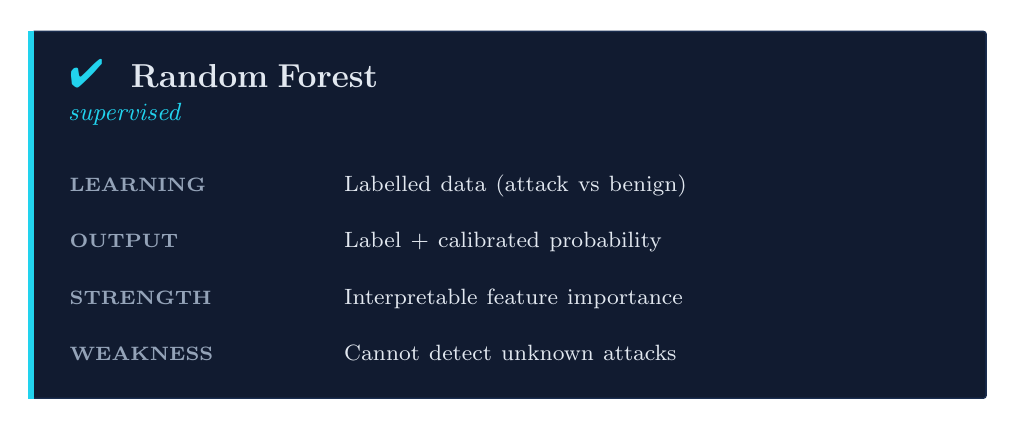
\begin{tikzpicture}
      \node[draw=navyborder,fill=navysurface,line width=0.5pt,rounded corners=1pt,
            inner sep=10pt,minimum width=\linewidth,minimum height=4.4cm,
            text width=0.92\linewidth,align=left] (t) {
        {\color{cyan2}\Large\ding{52}}\quad{\color{textmain}\bfseries\large Random Forest}\\
        {\color{cyan2}\itshape\small supervised}\\[6pt]
        \begin{tabular}{@{}p{0.30\linewidth}@{\hspace{4pt}}p{0.62\linewidth}@{}}
          {\color{textmute}\bfseries\fontsize{7}{8}\selectfont LEARNING}  & {\color{textmain}\fontsize{8.5}{10}\selectfont Labelled data (attack vs benign)} \\[2pt]
          {\color{textmute}\bfseries\fontsize{7}{8}\selectfont OUTPUT}    & {\color{textmain}\fontsize{8.5}{10}\selectfont Label + calibrated probability} \\[2pt]
          {\color{textmute}\bfseries\fontsize{7}{8}\selectfont STRENGTH}  & {\color{textmain}\fontsize{8.5}{10}\selectfont Interpretable feature importance} \\[2pt]
          {\color{textmute}\bfseries\fontsize{7}{8}\selectfont WEAKNESS}  & {\color{textmain}\fontsize{8.5}{10}\selectfont Cannot detect unknown attacks} \\
        \end{tabular}
      };
      \draw[line width=2.2pt,cyan2] (t.north west) -- (t.south west);
    \end{tikzpicture}

    \column{0.49\textwidth}
    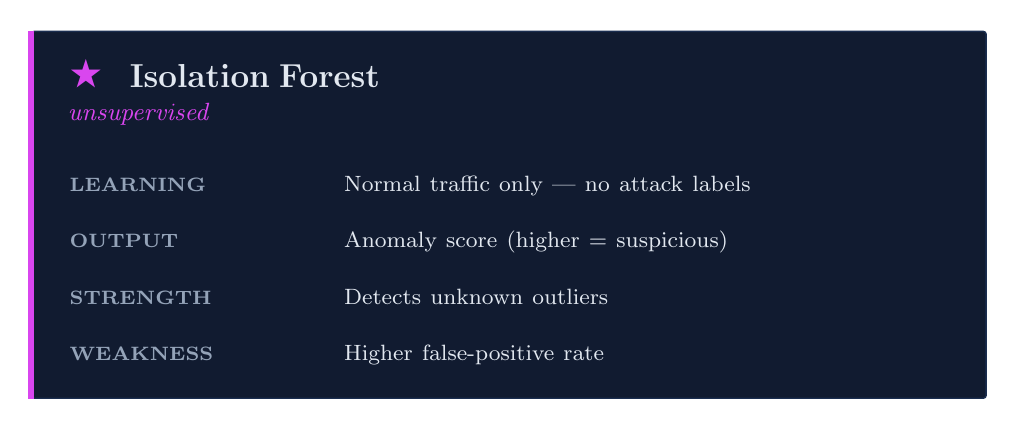
\begin{tikzpicture}
      \node[draw=navyborder,fill=navysurface,line width=0.5pt,rounded corners=1pt,
            inner sep=10pt,minimum width=\linewidth,minimum height=4.4cm,
            text width=0.92\linewidth,align=left] (t) {
        {\color{fuchsia2}\Large\ding{72}}\quad{\color{textmain}\bfseries\large Isolation Forest}\\
        {\color{fuchsia2}\itshape\small unsupervised}\\[6pt]
        \begin{tabular}{@{}p{0.30\linewidth}@{\hspace{4pt}}p{0.62\linewidth}@{}}
          {\color{textmute}\bfseries\fontsize{7}{8}\selectfont LEARNING}  & {\color{textmain}\fontsize{8.5}{10}\selectfont Normal traffic only — no attack labels} \\[2pt]
          {\color{textmute}\bfseries\fontsize{7}{8}\selectfont OUTPUT}    & {\color{textmain}\fontsize{8.5}{10}\selectfont Anomaly score (higher = suspicious)} \\[2pt]
          {\color{textmute}\bfseries\fontsize{7}{8}\selectfont STRENGTH}  & {\color{textmain}\fontsize{8.5}{10}\selectfont Detects unknown outliers} \\[2pt]
          {\color{textmute}\bfseries\fontsize{7}{8}\selectfont WEAKNESS}  & {\color{textmain}\fontsize{8.5}{10}\selectfont Higher false-positive rate} \\
        \end{tabular}
      };
      \draw[line width=2.2pt,fuchsia2] (t.north west) -- (t.south west);
    \end{tikzpicture}
  \end{columns}

  \vspace{0.5em}
  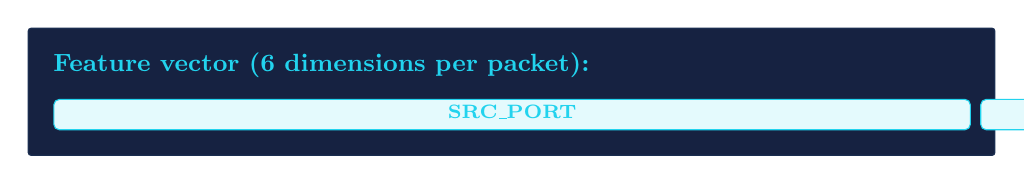
\begin{tikzpicture}
    \node[draw=navyborder,fill=navy2,line width=0.5pt,rounded corners=1pt,
          inner sep=9pt,minimum width=\linewidth,
          text width=0.96\linewidth,align=left] {
      {\color{cyan2}\bfseries\small Feature vector (6 dimensions per packet):}\\[5pt]
      \makebox[\linewidth][s]{%
        \tagchip{cyan2}{src\_port}\hfill
        \tagchip{cyan2}{dst\_port}\hfill
        \tagchip{cyan2}{length}\hfill
        \tagchip{cyan2}{proto\_id}\hfill
        \tagchip{cyan2}{flag\_mask}\hfill
        \tagchip{cyan2}{inter\_arrival\_ms}
      }
    };
  \end{tikzpicture}
\end{frame}

% --------------------------------------------------------------------
% SLIDE 9 — Forensics
% --------------------------------------------------------------------
\begin{frame}
  \frametitle{Per-alert capture}
  \framesubtitle{08 · Forensics}

  \begin{columns}[T,onlytextwidth]
    \column{0.55\textwidth}
    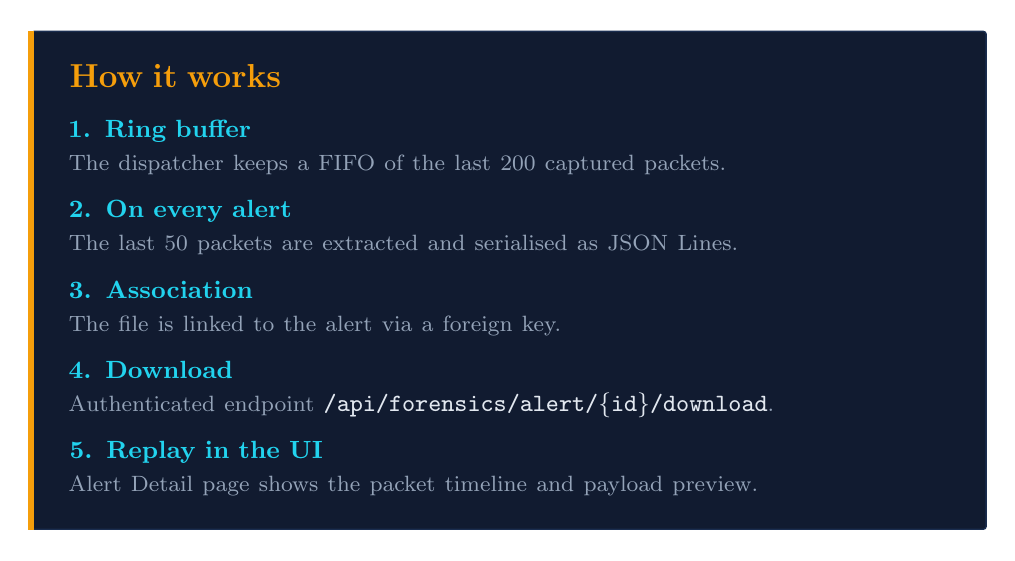
\begin{tikzpicture}
      \node[draw=navyborder,fill=navysurface,line width=0.5pt,rounded corners=1pt,
            inner sep=12pt,minimum width=\linewidth,minimum height=5.5cm,
            text width=0.92\linewidth,align=left] (t) {
        {\color{amber2}\bfseries\large How it works}\\[6pt]
        {\color{cyan2}\bfseries\small 1. Ring buffer}\\
        {\color{textmute}\fontsize{8}{10}\selectfont The dispatcher keeps a FIFO of the last 200 captured packets.}\\[5pt]
        {\color{cyan2}\bfseries\small 2. On every alert}\\
        {\color{textmute}\fontsize{8}{10}\selectfont The last 50 packets are extracted and serialised as JSON Lines.}\\[5pt]
        {\color{cyan2}\bfseries\small 3. Association}\\
        {\color{textmute}\fontsize{8}{10}\selectfont The file is linked to the alert via a foreign key.}\\[5pt]
        {\color{cyan2}\bfseries\small 4. Download}\\
        {\color{textmute}\fontsize{8}{10}\selectfont Authenticated endpoint \tmono{/api/forensics/alert/\{id\}/download}.}\\[5pt]
        {\color{cyan2}\bfseries\small 5. Replay in the UI}\\
        {\color{textmute}\fontsize{8}{10}\selectfont Alert Detail page shows the packet timeline and payload preview.}
      };
      \draw[line width=2.2pt,amber2] (t.north west) -- (t.south west);
    \end{tikzpicture}

    \column{0.42\textwidth}
    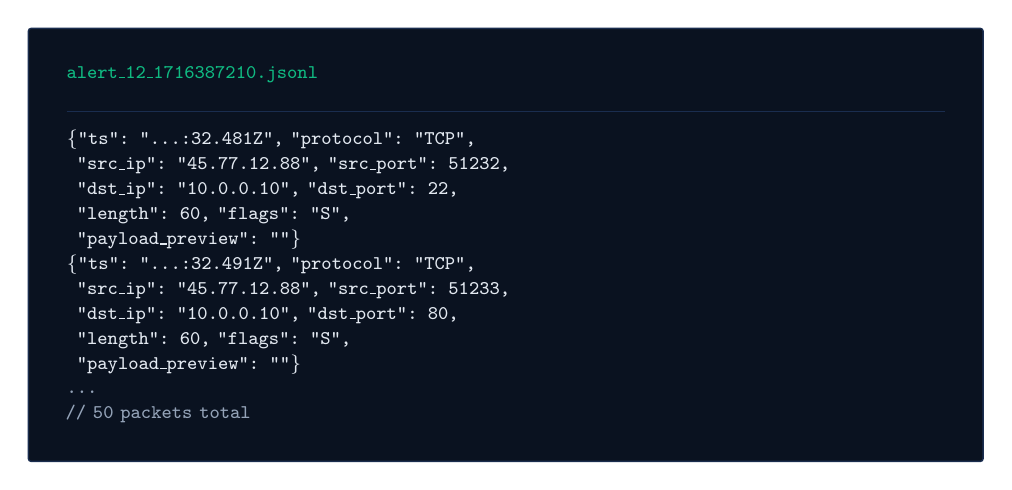
\begin{tikzpicture}
      \node[draw=navyborder,fill=navybg,line width=0.5pt,rounded corners=1pt,
            inner sep=10pt,minimum width=\linewidth,minimum height=5.5cm,
            text width=0.92\linewidth,align=left,font=\ttfamily\fontsize{7}{9}\selectfont] {
        {\color{green2}\bfseries alert\_12\_1716387210.jsonl}\\[3pt]
        \textcolor{navyborder}{\rule{\linewidth}{0.4pt}}\\[3pt]
        {\color{textmain}\{"ts": "...:32.481Z", "protocol": "TCP",}\\
        {\color{textmain}\hspace{0.5em}"src\_ip": "45.77.12.88", "src\_port": 51232,}\\
        {\color{textmain}\hspace{0.5em}"dst\_ip": "10.0.0.10", "dst\_port": 22,}\\
        {\color{textmain}\hspace{0.5em}"length": 60, "flags": "S",}\\
        {\color{textmain}\hspace{0.5em}"payload\_preview": ""\}}\\
        {\color{textmain}\{"ts": "...:32.491Z", "protocol": "TCP",}\\
        {\color{textmain}\hspace{0.5em}"src\_ip": "45.77.12.88", "src\_port": 51233,}\\
        {\color{textmain}\hspace{0.5em}"dst\_ip": "10.0.0.10", "dst\_port": 80,}\\
        {\color{textmain}\hspace{0.5em}"length": 60, "flags": "S",}\\
        {\color{textmain}\hspace{0.5em}"payload\_preview": ""\}}\\
        {\color{textmute}...}\\
        {\color{textmute}// 50 packets total}
      };
    \end{tikzpicture}
  \end{columns}
\end{frame}

% --------------------------------------------------------------------
% SLIDE 10 — Usage example: Dashboard + Attack Console (screenshots)
% --------------------------------------------------------------------
\begin{frame}
  \frametitle{Dashboard and Attack Console}
  \framesubtitle{09 · Usage example}

  \begin{columns}[T,onlytextwidth]
    \column{0.49\textwidth}
    \kicker{Dashboard}\\[3pt]
    \fbox{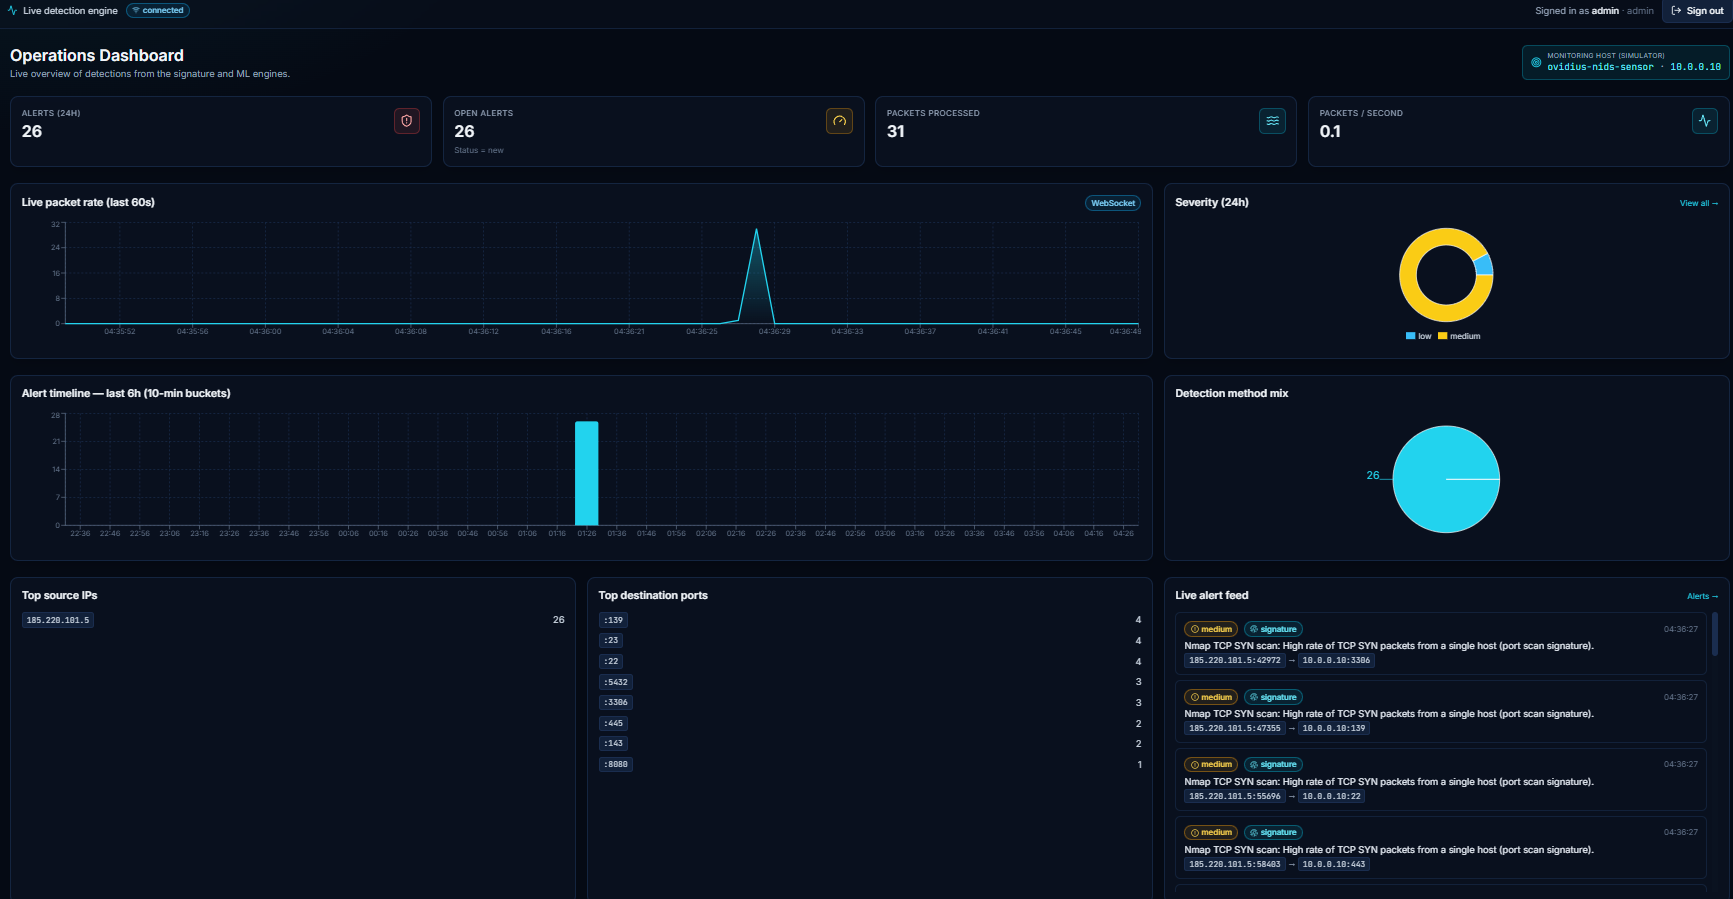
\includegraphics[width=\linewidth]{dashboard.png}}
    \vspace{2pt}\\
    {\color{textmute}\fontsize{7.5}{9}\selectfont Live KPIs, packet-rate chart, severity pie, alert timeline, live feed. Monitoring host \tmono{10.0.0.10}.}

    \column{0.49\textwidth}
    \kicker{Attack Console}\\[3pt]
    \fbox{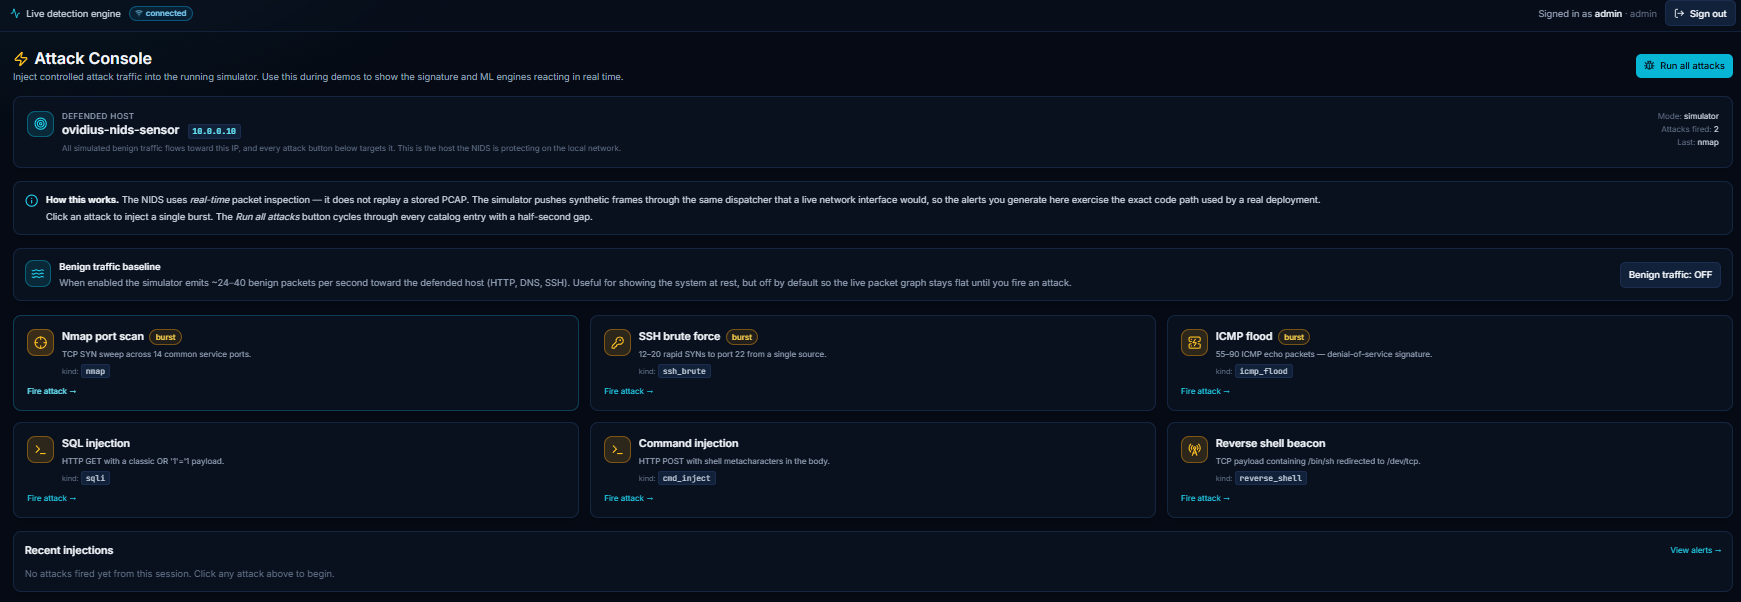
\includegraphics[width=\linewidth]{attack-console.png}}
    \vspace{2pt}\\
    {\color{textmute}\fontsize{7.5}{9}\selectfont Six attack buttons. Defended host + benign-traffic toggle. Recent injections audit trail.}
  \end{columns}
\end{frame}

% --------------------------------------------------------------------
% SLIDE 11 — Alert flow
% --------------------------------------------------------------------
\begin{frame}
  \frametitle{From attack to triage}
  \framesubtitle{10 · Alert flow}

  \begin{columns}[T,onlytextwidth]
    \column{0.49\textwidth}
    \tile{amber2}{1 · Attack triggered}{User clicks ``Nmap port scan'' in the Attack Console. The simulator generates 30 TCP SYN packets from \tmono{185.220.101.5} toward \tmono{10.0.0.10}.}
    \vspace{0.4em}
    \tile{green2}{3 · Signature detection}{After the 8th packet, the ``Nmap TCP SYN scan'' rule crosses the threshold (8 SYNs in 5\,s) — the alert is created.}
    \vspace{0.4em}
    \tile{blue2}{5 · Real-time notification}{\tmono{alert\_bus} publishes on WebSocket. Alerts page receives the alert instantly via \tmono{/ws/alerts}.}

    \column{0.49\textwidth}
    \tile{cyan2}{2 · Capture}{The dispatcher receives each packet, updates the ring buffer and publishes on \tmono{traffic\_bus} for the live chart.}
    \vspace{0.4em}
    \tile{fuchsia2}{4 · Persistence + forensics}{The alert is saved in SQLite. JSONL ring-tail with the last 50 packets written to disk and linked to the alert.}
    \vspace{0.4em}
    \tile{red2}{6 · Triage}{The analyst opens Alert Detail, sees the packet timeline and downloads the JSONL capture for investigation.}
  \end{columns}
\end{frame}

% --------------------------------------------------------------------
% SLIDE 12 — Competition
% --------------------------------------------------------------------
\begin{frame}
  \frametitle{Similar applications on the market}
  \framesubtitle{11 · Competition}

  \vspace{-0.5em}
  \scriptsize
  \begin{center}
  \renewcommand{\arraystretch}{0.78}
  \arrayrulecolor{navyborder}
  \begin{tabular}{@{}p{4.0cm}>{\centering\arraybackslash}p{0.85cm}>{\centering\arraybackslash}p{1.0cm}>{\centering\arraybackslash}p{0.85cm}>{\centering\arraybackslash}p{0.85cm}>{\centering\arraybackslash}p{0.85cm}>{\centering\arraybackslash}p{1.5cm}@{}}
    \toprule
    {\color{textmain}\bfseries Feature} &
    {\color{textmain}\bfseries Snort} &
    {\color{textmain}\bfseries Suricata} &
    {\color{textmain}\bfseries Zeek} &
    {\color{textmain}\bfseries Wazuh} &
    {\color{textmain}\bfseries Splunk} &
    {\color{cyan2}\bfseries Ovidius NIDS} \\
    \midrule
    {\color{textmain}Signature engine}           & {\color{green2}\ding{52}} & {\color{green2}\ding{52}} & {\color{amber2}$\sim$} & {\color{amber2}$\sim$} & {\color{amber2}$\sim$} & {\color{green2}\ding{52}} \\
    {\color{textmain}Machine Learning engine}    & {\color{red2}\ding{55}} & {\color{red2}\ding{55}} & {\color{red2}\ding{55}} & {\color{amber2}$\sim$} & {\color{green2}\ding{52}} & {\color{green2}\ding{52}} \\
    {\color{textmain}Hybrid category}            & {\color{textdim}--} & {\color{textdim}--} & {\color{textdim}--} & {\color{red2}\ding{55}} & {\color{red2}\ding{55}} & {\color{green2}\ding{52}} \\
    {\color{textmain}Built-in analyst UI}        & {\color{red2}\ding{55}} & {\color{red2}\ding{55}} & {\color{red2}\ding{55}} & {\color{green2}\ding{52}} & {\color{green2}\ding{52}} & {\color{green2}\ding{52}} \\
    {\color{textmain}Per-alert forensic capture} & {\color{red2}\ding{55}} & {\color{red2}\ding{55}} & {\color{red2}\ding{55}} & {\color{red2}\ding{55}} & {\color{red2}\ding{55}} & {\color{green2}\ding{52}} \\
    {\color{textmain}Real-time streaming in UI}  & {\color{red2}\ding{55}} & {\color{red2}\ding{55}} & {\color{red2}\ding{55}} & {\color{amber2}$\sim$} & {\color{green2}\ding{52}} & {\color{green2}\ding{52}} \\
    {\color{textmain}Rules editable from UI}     & {\color{red2}\ding{55}} & {\color{red2}\ding{55}} & {\color{red2}\ding{55}} & {\color{green2}\ding{52}} & {\color{green2}\ding{52}} & {\color{green2}\ding{52}} \\
    {\color{textmain}One-click deploy}           & {\color{red2}\ding{55}} & {\color{red2}\ding{55}} & {\color{red2}\ding{55}} & {\color{red2}\ding{55}} & {\color{red2}\ding{55}} & {\color{green2}\ding{52}} \\
    {\color{textmain}Open source · free}         & {\color{green2}\ding{52}} & {\color{green2}\ding{52}} & {\color{green2}\ding{52}} & {\color{green2}\ding{52}} & {\color{red2}\ding{55}} & {\color{green2}\ding{52}} \\
    \bottomrule
  \end{tabular}
  \end{center}

  \vspace{0.2em}
  \begin{center}
  
\begin{tikzpicture}
    \node[draw=cyan2,fill=navysurface,line width=0.6pt,rounded corners=1pt,
          inner sep=5pt,text width=0.95\textwidth,align=center,
          font=\scriptsize\itshape] {
      {\color{textmain}\textbf{All in one binary} — detection, ML, forensics and UI; \textbf{forensics built-in} per alert; \textbf{explicit hybrid} category; \textbf{five-minute demo} via one-click launcher.}
    };
  \end{tikzpicture}
  \end{center}
\end{frame}

% --------------------------------------------------------------------
% SLIDE 13 — Conclusions
% --------------------------------------------------------------------
\begin{frame}
  \frametitle{What was achieved}
  \framesubtitle{12 · Conclusions}

  \begin{columns}[T,onlytextwidth]
    \column{0.32\textwidth}
    \tile{green2}{\ding{52}~End-to-end functional}{Capture, hybrid detection, forensics, auth, live dashboard — all operational.}
    \vspace{0.4em}
    \tile{amber2}{\ding{73}~Forensics on disk}{Per alert: JSONL with the last 50 packets, authenticated download from UI.}

    \column{0.32\textwidth}
    \tile{cyan2}{\ding{110}~Real-time, low latency}{<\,1\,ms per packet at signature engine, <\,250\,ms total to UI.}
    \vspace{0.4em}
    \tile{cyan2}{\ding{229}~One-click deployment}{\tmono{run.bat} / \tmono{run.sh} / \tmono{run.py} — auto install + start.}

    \column{0.32\textwidth}
    \tile{fuchsia2}{\ding{72}~ML trainable from UI}{Random Forest and Isolation Forest, metrics and feature importance.}
    \vspace{0.4em}
    \tile{blue2}{\textbf{<\hspace{-1pt}\textgreater}~Extensible code}{Rules editable without restart. Decoupled modules. Auto OpenAPI.}
  \end{columns}
\end{frame}

% --------------------------------------------------------------------
% SLIDE 14 — Future Work
% --------------------------------------------------------------------
\begin{frame}
  \frametitle{What is left for future development}
  \framesubtitle{13 · Future work}

  \begin{columns}[T,onlytextwidth]
    \column{0.49\textwidth}
    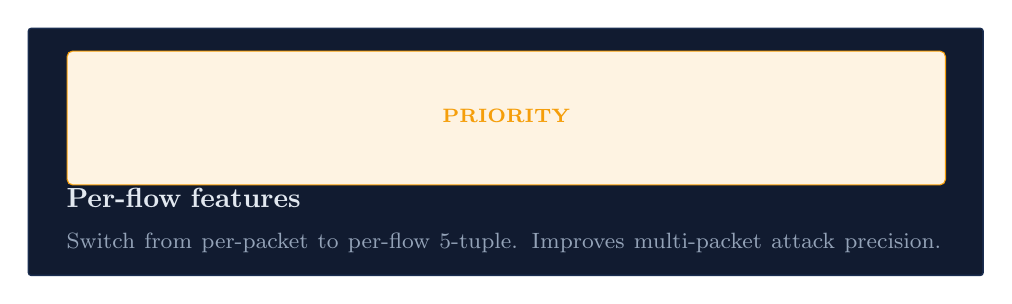
\begin{tikzpicture}
      \node[draw=navyborder,fill=navysurface,line width=0.5pt,rounded corners=1pt,
            inner sep=8pt,minimum width=\linewidth,minimum height=1.7cm,
            text width=0.92\linewidth,align=left] {
        \tagchip{amber2}{Priority}\quad{\color{textmain}\bfseries Per-flow features}\\[3pt]
        {\color{textmute}\fontsize{8}{10}\selectfont Switch from per-packet to per-flow 5-tuple. Improves multi-packet attack precision.}
      };
    \end{tikzpicture}
    \vspace{0.3em}
    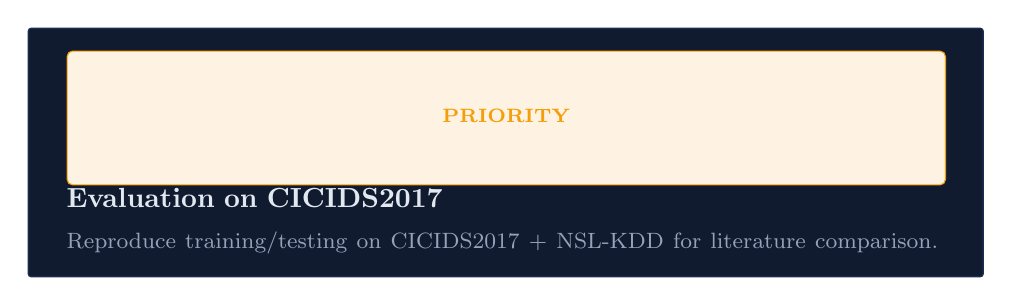
\begin{tikzpicture}
      \node[draw=navyborder,fill=navysurface,line width=0.5pt,rounded corners=1pt,
            inner sep=8pt,minimum width=\linewidth,minimum height=1.7cm,
            text width=0.92\linewidth,align=left] {
        \tagchip{amber2}{Priority}\quad{\color{textmain}\bfseries Evaluation on CICIDS2017}\\[3pt]
        {\color{textmute}\fontsize{8}{10}\selectfont Reproduce training/testing on CICIDS2017 + NSL-KDD for literature comparison.}
      };
    \end{tikzpicture}
    \vspace{0.3em}
    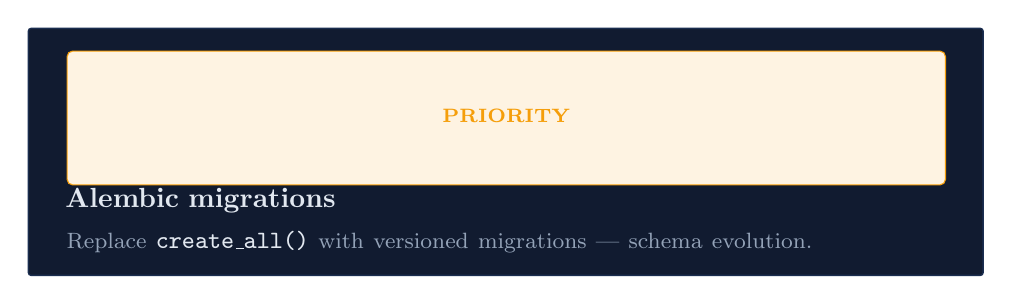
\begin{tikzpicture}
      \node[draw=navyborder,fill=navysurface,line width=0.5pt,rounded corners=1pt,
            inner sep=8pt,minimum width=\linewidth,minimum height=1.7cm,
            text width=0.92\linewidth,align=left] {
        \tagchip{amber2}{Priority}\quad{\color{textmain}\bfseries Alembic migrations}\\[3pt]
        {\color{textmute}\fontsize{8}{10}\selectfont Replace \tmono{create\_all()} with versioned migrations — schema evolution.}
      };
    \end{tikzpicture}

    \column{0.49\textwidth}
    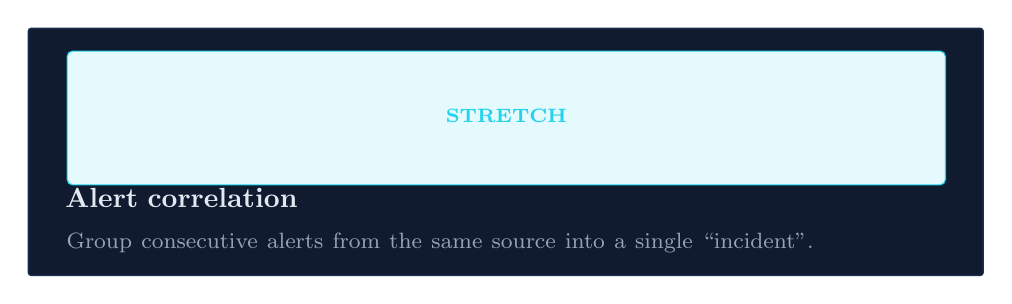
\begin{tikzpicture}
      \node[draw=navyborder,fill=navysurface,line width=0.5pt,rounded corners=1pt,
            inner sep=8pt,minimum width=\linewidth,minimum height=1.7cm,
            text width=0.92\linewidth,align=left] {
        \tagchip{cyan2}{Stretch}\quad{\color{textmain}\bfseries Alert correlation}\\[3pt]
        {\color{textmute}\fontsize{8}{10}\selectfont Group consecutive alerts from the same source into a single ``incident''.}
      };
    \end{tikzpicture}
    \vspace{0.3em}
    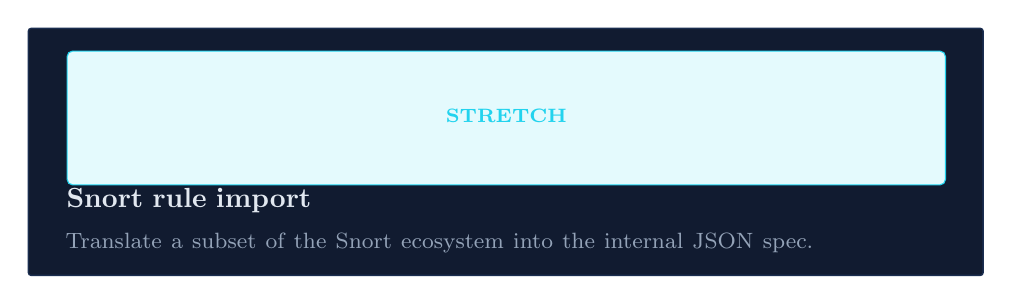
\begin{tikzpicture}
      \node[draw=navyborder,fill=navysurface,line width=0.5pt,rounded corners=1pt,
            inner sep=8pt,minimum width=\linewidth,minimum height=1.7cm,
            text width=0.92\linewidth,align=left] {
        \tagchip{cyan2}{Stretch}\quad{\color{textmain}\bfseries Snort rule import}\\[3pt]
        {\color{textmute}\fontsize{8}{10}\selectfont Translate a subset of the Snort ecosystem into the internal JSON spec.}
      };
    \end{tikzpicture}
    \vspace{0.3em}
    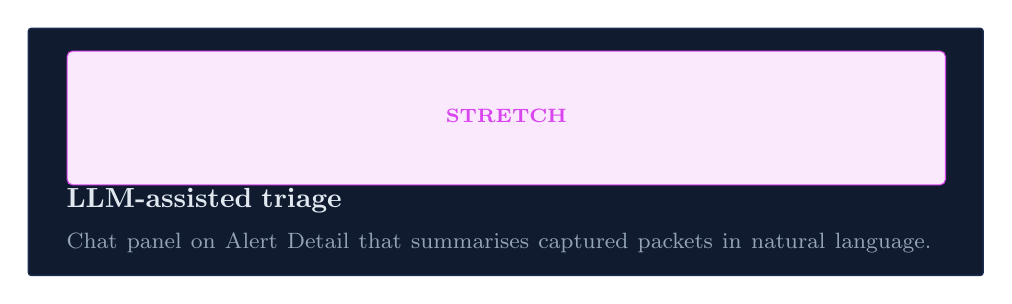
\begin{tikzpicture}
      \node[draw=navyborder,fill=navysurface,line width=0.5pt,rounded corners=1pt,
            inner sep=8pt,minimum width=\linewidth,minimum height=1.7cm,
            text width=0.92\linewidth,align=left] {
        \tagchip{fuchsia2}{Stretch}\quad{\color{textmain}\bfseries LLM-assisted triage}\\[3pt]
        {\color{textmute}\fontsize{8}{10}\selectfont Chat panel on Alert Detail that summarises captured packets in natural language.}
      };
    \end{tikzpicture}
  \end{columns}
\end{frame}

% --------------------------------------------------------------------
% SLIDE 15 — Thank you
% --------------------------------------------------------------------
{
\setbeamertemplate{footline}{}
\begin{frame}[plain]
  \vfill
  \begin{center}
    {\color{cyan2}\fontsize{60}{72}\selectfont\ding{52}}\\[0.3em]
    \tikz \draw[cyan2,line width=1.2pt] (0,0) -- (5,0);\\[0.5em]
    {\color{textmain}\bfseries\fontsize{36}{42}\selectfont Thank you for your attention!}
  \end{center}
  \vfill
  \begin{center}
    {\color{textdim}\small Bora Cristian-Vasile  \,$\cdot$\,  Universitatea OVIDIUS din Constanța  \,$\cdot$\,  Iulie 2026}
  \end{center}
\end{frame}
}

\end{document}
